\subsection{Inverting Zero-Crossing Level Detector With Hysteresis:}

Setting the {\itshape waveform generator} in a sinusoidal signal with a frequency of 1 KHz and 16 $V_{pp}$ we connect the positive terminal of the {\itshape generator} to the $V_{i}$ terminal of the circuit in Figure 3.3.0 and the negative terminal to the common ground. Then, once the respectively sources in the terminals 7 and 4 were connected, we turned on the {\itshape generator} and the voltage sources, thus, connecting the channel 1 of the oscilloscope in $V_{i}$ and the channel 2 in the $V_{o}$ we registered the waveform in Figure 3.3.1. Finally, we change the oscilloscope mode to X-Y and captured the transfer function in Figure 3.3.2. \hfill \break

\begin{figure}[H]
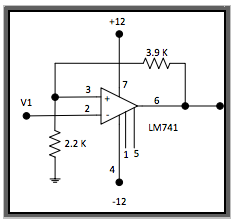
\includegraphics[width = 8cm, height = 6cm]{c3.png}
\centering \linebreak \linebreak Figure 3.3.0: Inverting zero-crossing level detector with hysteresis.
\end{figure} \hfill

\begin{multicols}{2}
\begin{figure}[H]
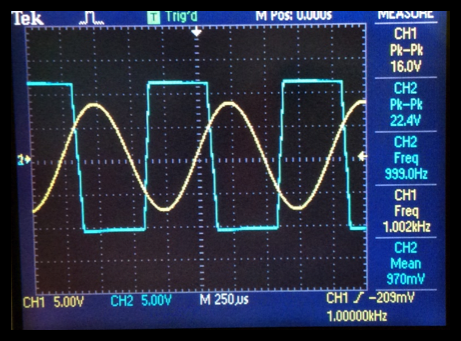
\includegraphics[width = 8cm, height = 5cm]{o3.png}
\centering \linebreak \linebreak Figure 3.3.1: Input and output waveform.
\end{figure} \hfill

\begin{figure}[H]

\includegraphics[width = 8cm, height = 5cm]{t3.png}
\centering \linebreak \linebreak Figure 3.3.2: Transfer function for Figure 3.3.1
\end{figure} \hfill
\end{multicols} 

{\bfseries\itshape\color{carmine}{Observation:}} {\itshape\color{carmine}{In Figure 3.3.1 we can see two waveform, the yellow one it's the input of the circuit, analogously, the blue it's for the output.}}

\pagebreak